Como mencionamos, nos interesa saber que heuristica de búsqueda local se adapta mejor a cada tipo de entrada estudiada con el algoritmo del ejercicio 2. Para esto, las enunciaremos nuevamente:

\begin{enumerate}
\item No se obtiene soluci\'on por no haber las pokeparadas necesarias para ganar en todos los gimnasios.
\item No se obtiene soluci\'on ya que la capacidad de la mochila no puede contener las pociones necesarias para vencer a un cierto gimnasio.
\item Todos los gimnasios sin necesidad de pociones para ser vencidos.
\item Las pokeparadas y los gimnasios se reciben en orden de la forma en la cual exista una pokeparada puntual para ir a cada gimnasio
\end{enumerate}

Veremos para cada una de las familias enunciadas, cual de las búsquedas locales nos provee una solución mejor a la solución provista por el algoritmo $greedy$. O en caso de no proveer ninguna solución, trataremos de dar respuesta a los motivos.

Para cada búsqueda local, se tomará una media alfa podada con $\alpha$ = 0.5 de manera de podar un 25\% de los datos a cada lado. De esta forma no habrá outliers en las muestras consideradas. 
La cantidad de mediciones para tomar la media será de 30. Además se tomará la varianza muestral usando la media calculada y las mediciones que queden luego de aplicar la media.\\

\subsubsection*{Familia 1}

\vspace*{0.3cm} \vspace*{0.3cm}
  \begin{center}
 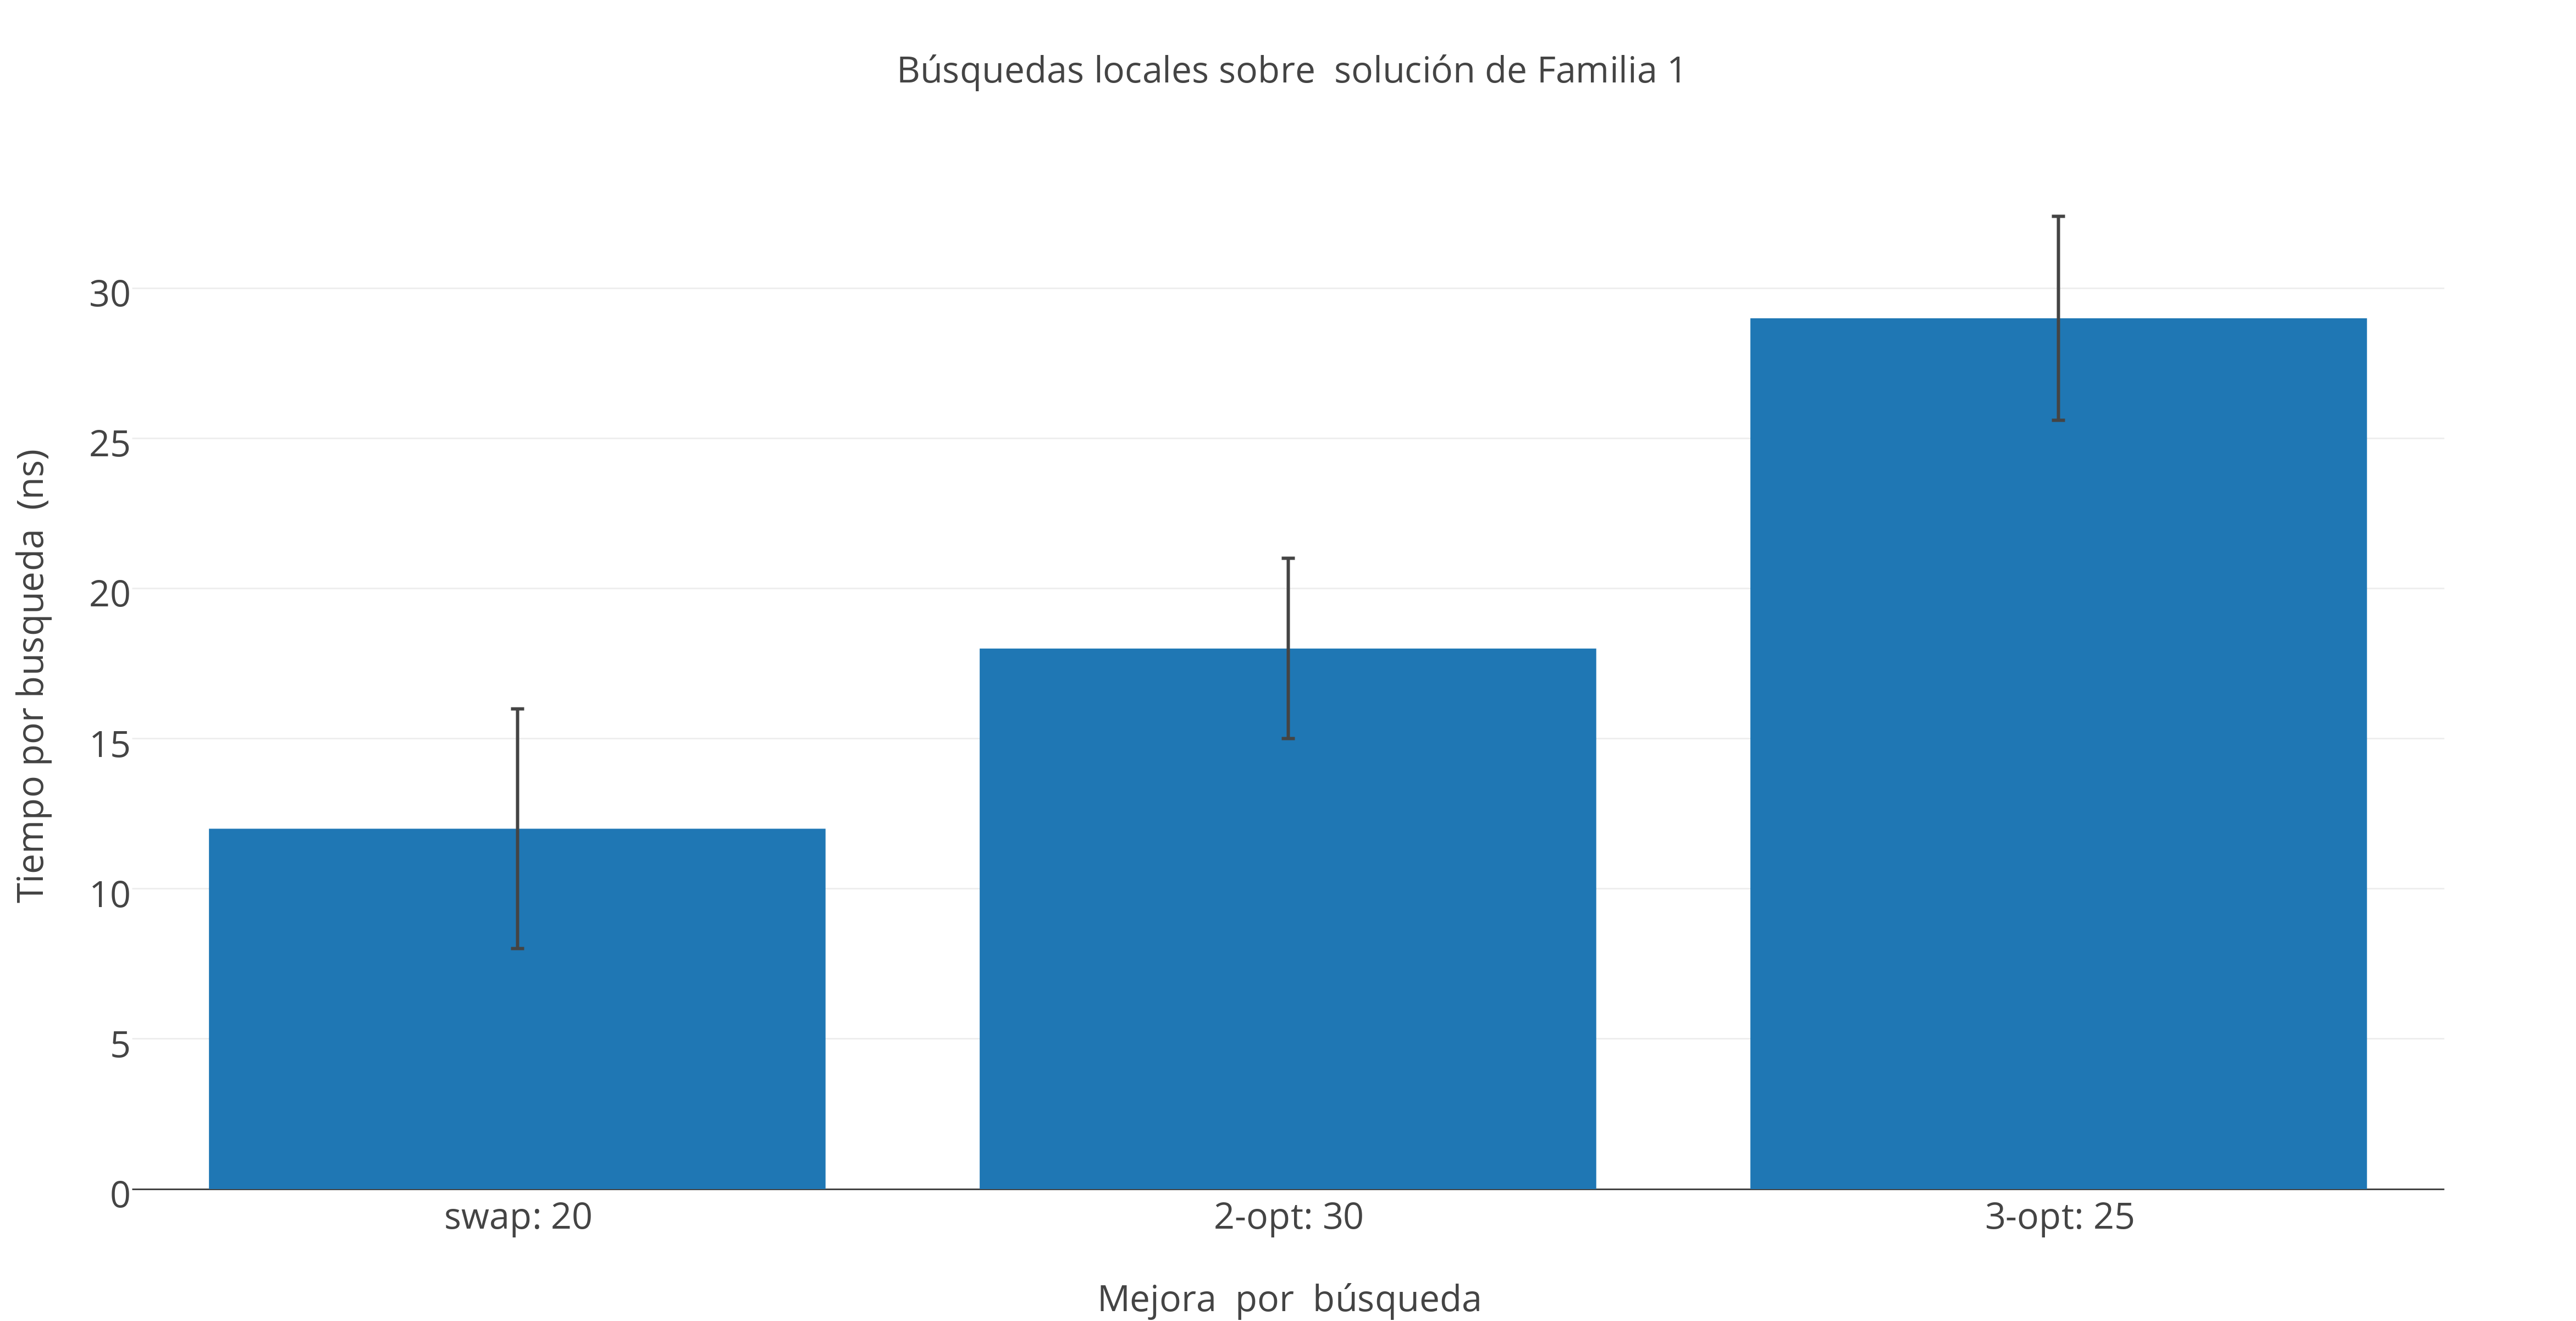
\includegraphics[scale=0.5]{./EJ3/local_search_familia.png}
 {            \textit{Gráfico \ 3.1 - Búsquedas locales sobre Familia 1}}
  \end{center}
  \vspace*{0.3cm}

\subsubsection*{Familia 2}

\vspace*{0.3cm} \vspace*{0.3cm}
  \begin{center}
 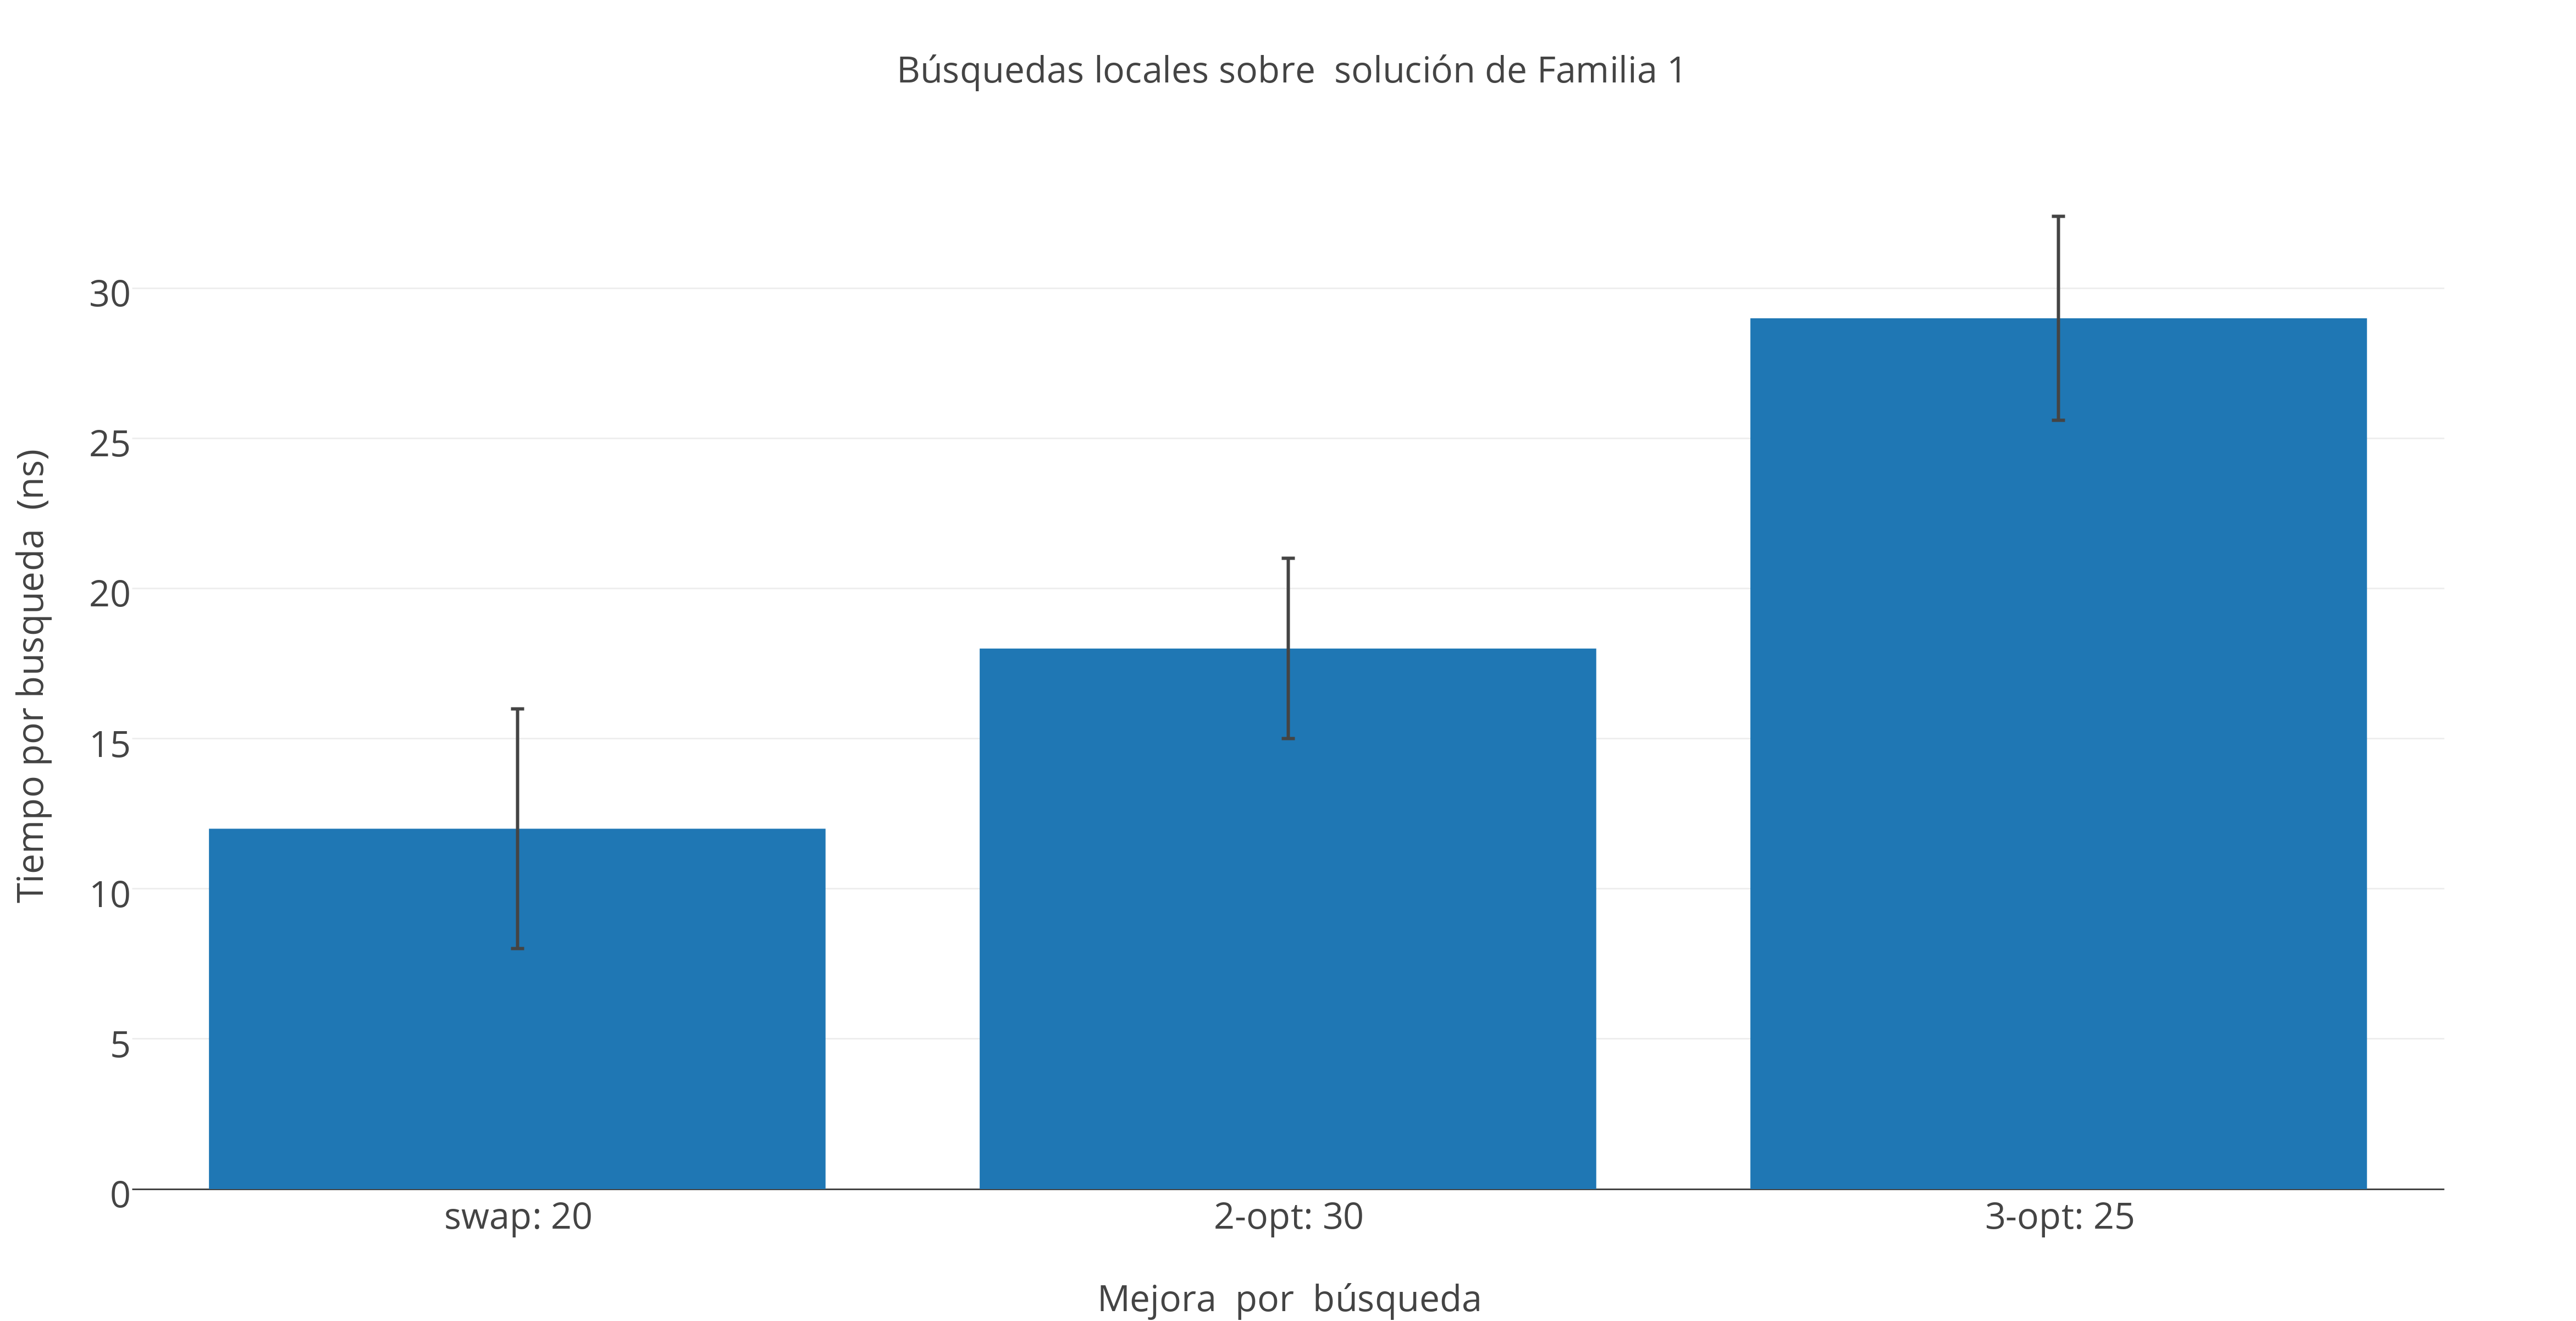
\includegraphics[scale=0.5]{./EJ3/local_search_familia.png}
 {            \textit{Gráfico \ 3.2 - Búsquedas locales sobre Familia 2}}
  \end{center}
  \vspace*{0.3cm}

\subsubsection*{Familia 3}

\vspace*{0.3cm} \vspace*{0.3cm}
  \begin{center}
 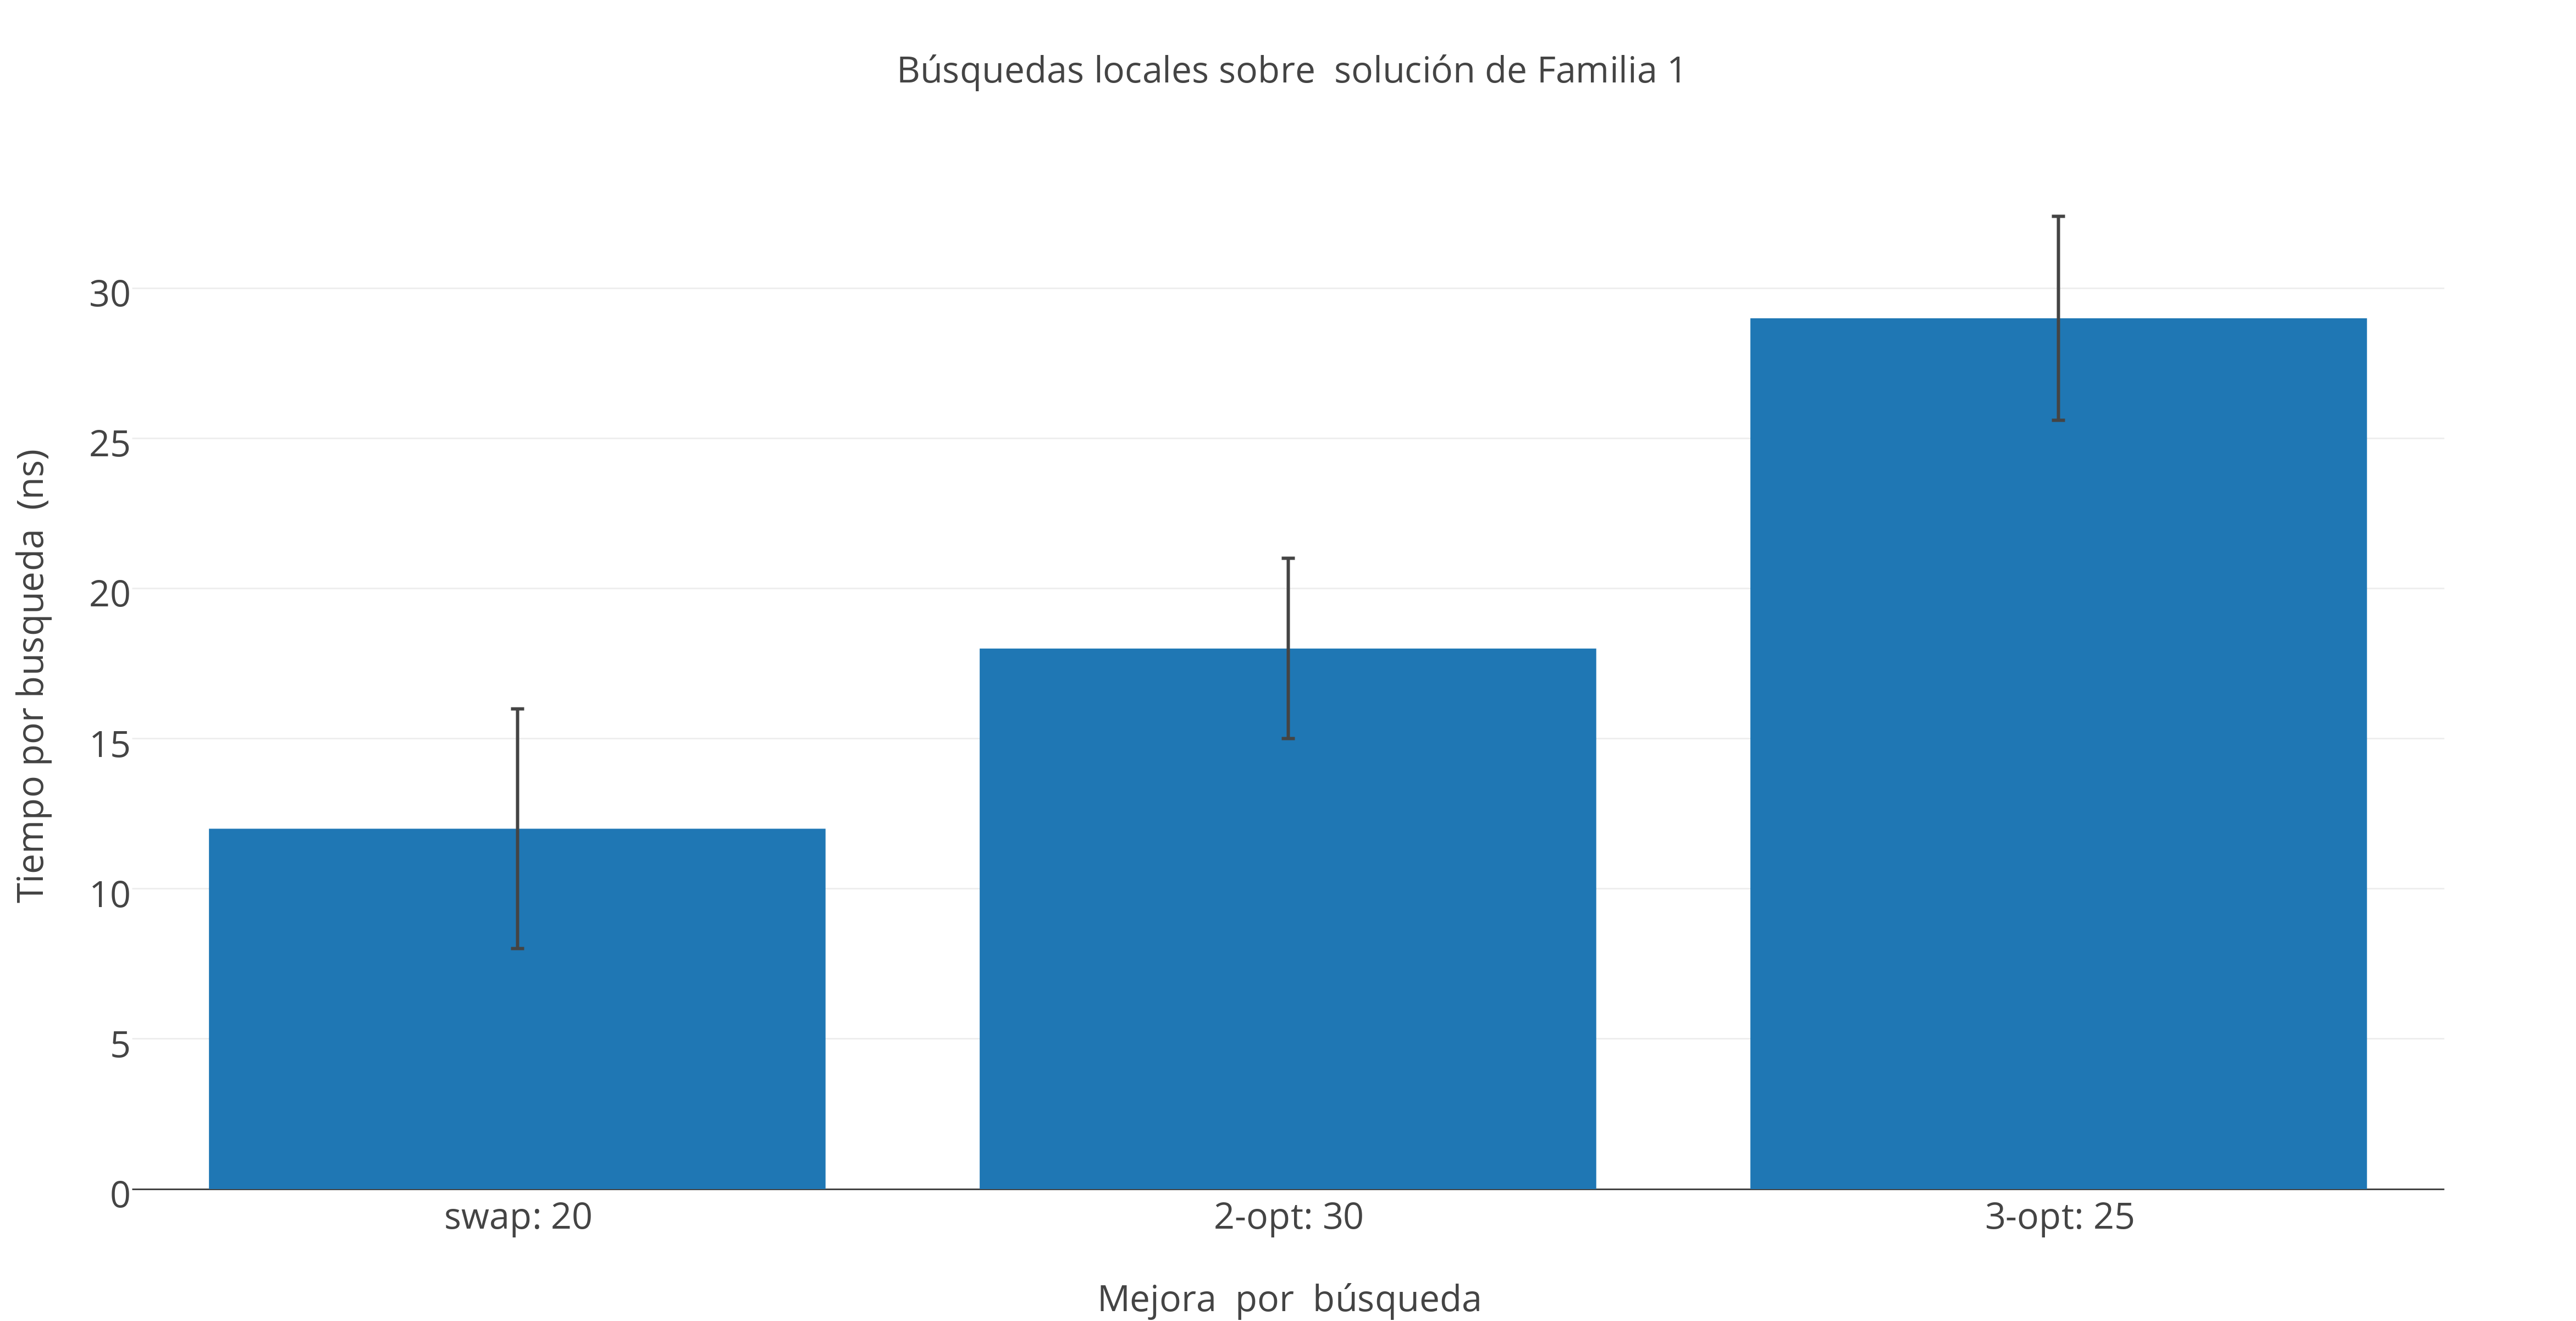
\includegraphics[scale=0.5]{./EJ3/local_search_familia.png}
 {            \textit{Gráfico \ 3.3 - Búsquedas locales sobre Familia 3}}
  \end{center}
  \vspace*{0.3cm}

\subsubsection*{Familia 4}

\vspace*{0.3cm} \vspace*{0.3cm}
  \begin{center}
 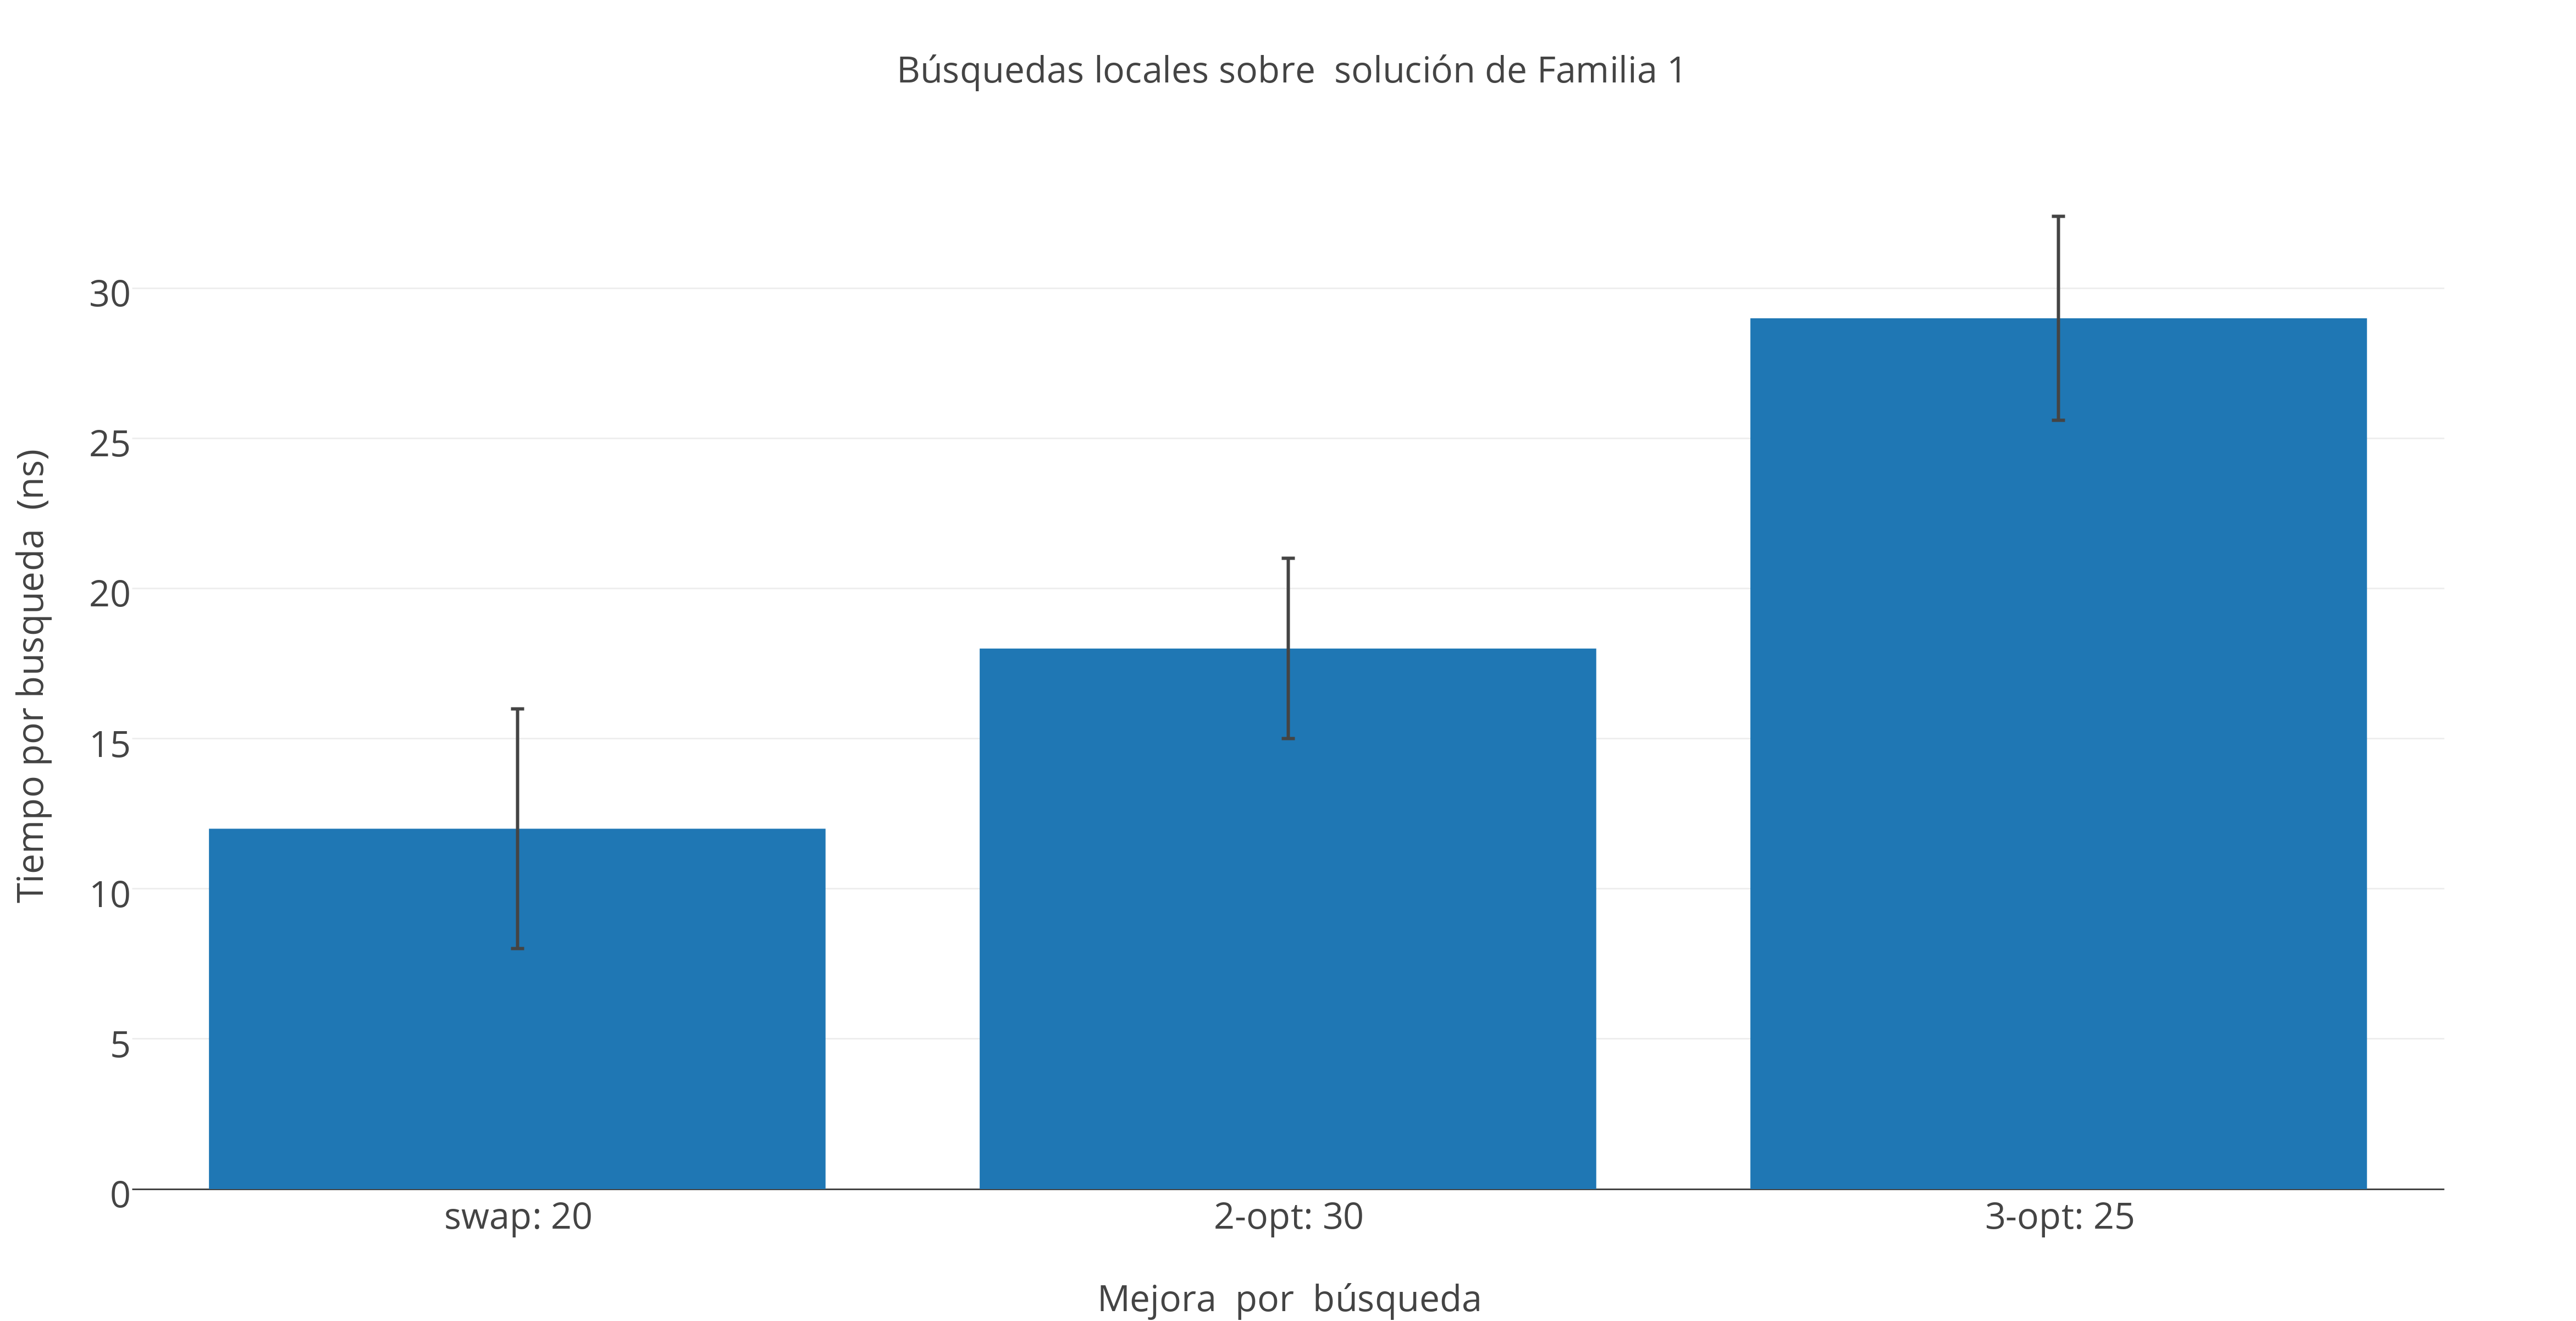
\includegraphics[scale=0.5]{./EJ3/local_search_familia.png}
 {            \textit{Gráfico \ 3.4 - Búsquedas locales sobre Familia 4}}
  \end{center}
  \vspace*{0.3cm}
